\section{Runtime View}
\subsection{Runtime Overview}

\begin{figure}[ht]
	\centering
	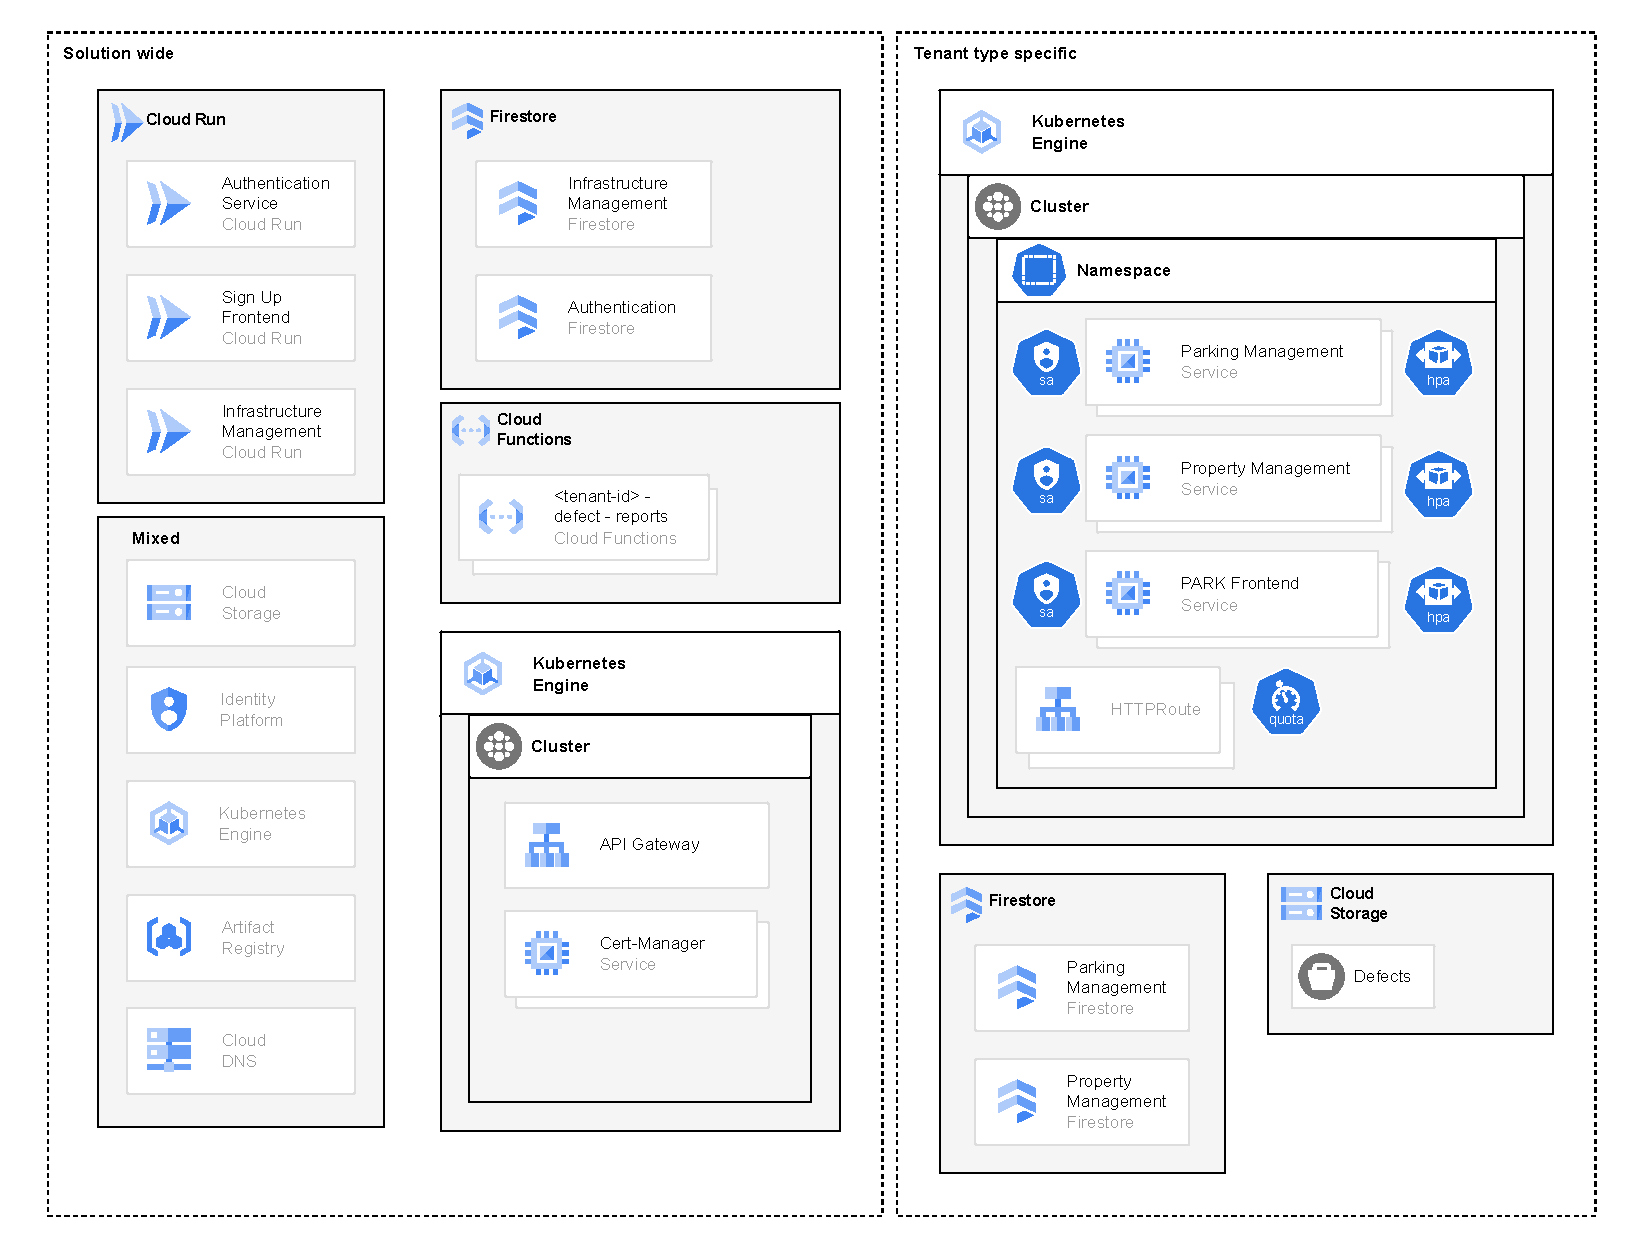
\includegraphics[width=\textwidth]{resources/03-runtime-view/pdf/cloud-ressources.pdf}
	\caption{Übersicht über die Cloud Ressourcen}
	\label{fig:cloud-ressources}
\end{figure}

\begin{figure}[ht]
	\centering
	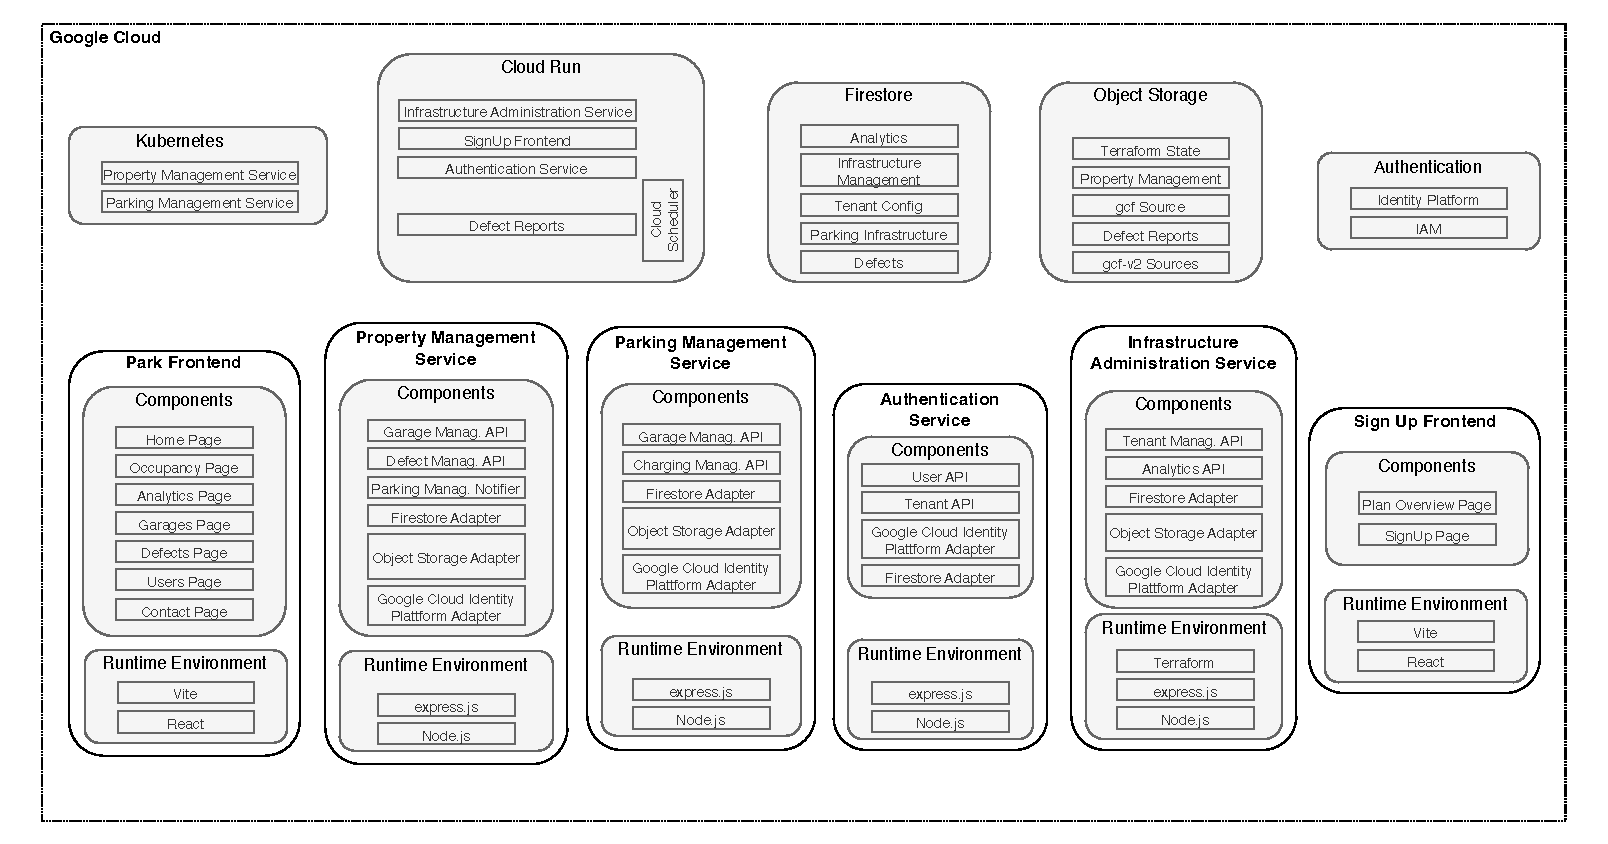
\includegraphics[width=\textwidth]{resources/03-runtime-view/pdf/architecture.pdf}
	\caption{Alle Mircoservices}
	\label{fig:system-architecture}
\end{figure}

In Abbildung~\ref{fig:cloud-ressources} werden alle verwendeten Cloud Ressourcen unterteilt in zwei Gruppen dargestellt:
\paragraph{Anwendungweite Ressources} sind Ressourcen, die von allen Tenants gemeinsam genutzt werden.
Diese Ressourcen unterteilen sich nochmal in folgende Kategorien:
\begin{itemize}
	\item \textbf{Cloud Run} - Alle Services, welche in Cloud Run laufen. (Authentication Service, Infrastructure Management Service \& Sign Up Frontend)
	\item \textbf{Firestore} - Die Firestore Datenbanken, welche von den Cloud Run Services benötigt werden.
	\item \textbf{Cloud Functions} - Pro Tenant gibt es eine Defect-Report Cloud Function.
	\item \textbf{Mixed} - Weitere Cloud Ressourcen, welche für den Betrieb unsere Anwendung benötigt werden. (z.B. Cloud Storage, Identity Platform, Kubernetes Engine, Artifact Registry \& Ingres / DNS)
\end{itemize}

\paragraph{Tenant Typ spezifische Ressources} sind Ressourcen, die sich von allen Tenants des selben Tenant Typs geteilt werden.
Jeder Enterprise Tenant wird hierbei als eigener Tenant Typ betrachtet, um die verwendeten Ressourcen bessere darstellen und erklären zu können.
Die Ressourcen unterteilen sich nochmal in folgende Kategorien:
\begin{itemize}
	\item \textbf{Kubernetes} - Innerhalb der annwedungsweiten Kubernetes Engine existiert ein Cluster. Innerhalb des Cluster wird pro Tenant Typ ein neuer Namespace angelegt, in welchem die Services (Property Management \& Parking Management) laufen, welche sich alle Tenants eines Typs teilen.
	\item \textbf{Firestore} - Die Firestore Datenbanken, welche für die Services im Tenant Typ spezifischen Namespace benötigt werden. (Property Management \& Parking Management)
	\item \textbf{Cloud Storage} - Für den Property Management Service wird ein eigener Bucket angelegt, um die Bilder der Defects speichern zu können.
\end{itemize}

Um die Interaktionen zwischen den Komponenten als auch den anwendungweiten und Tenant Typ spezifischen Ressourcen zu verdeutlichen, wird in Abbildung~\ref{fig:system-architecture} die gesamte Systemarchitektur dargestellt. Hier sieht man, wie sich alle Komponenten eine Authentication Service und Infrastructure Management Service Instanz teilen.

\begin{figure}[ht]
	\centering
	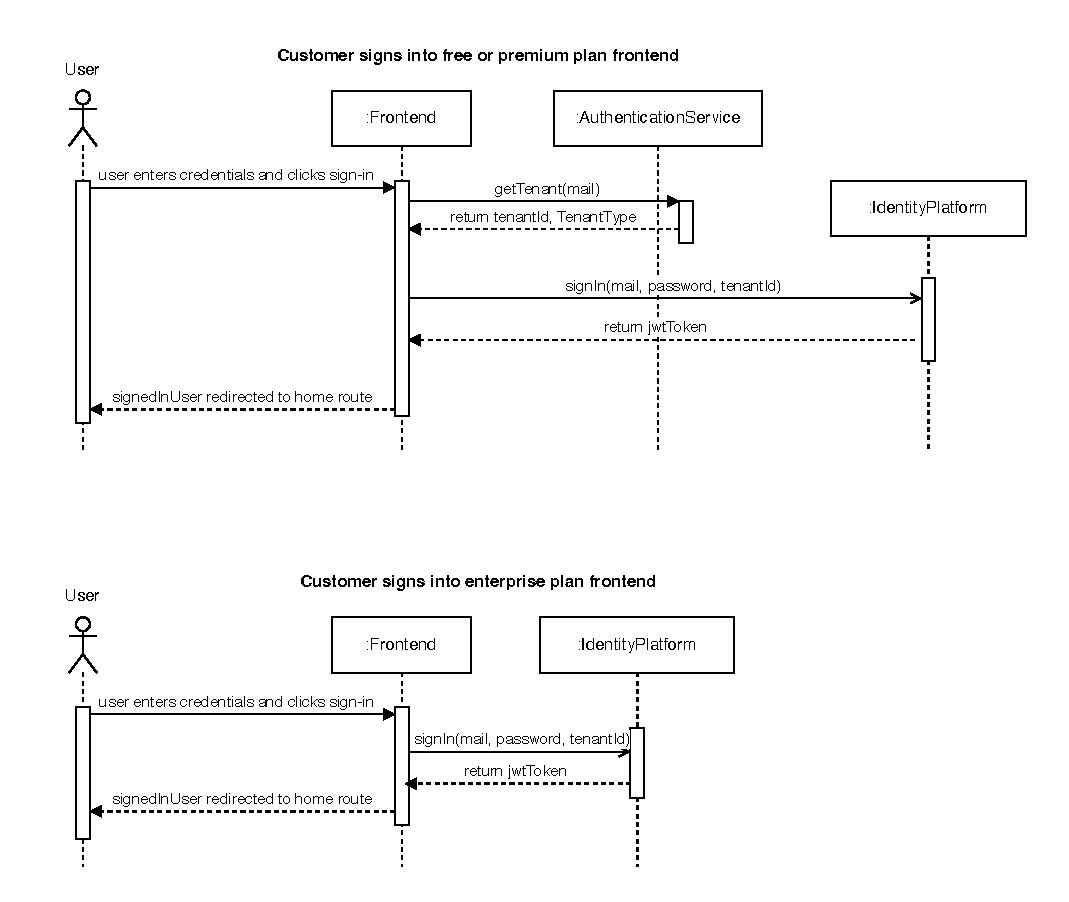
\includegraphics[width=\textwidth]{resources/03-runtime-view/pdf/authentication-sequence.pdf}
	\caption{Ablauf der Tenant Typ abhängigen Authentifizierung}
	\label{fig:authentication-sequence}
\end{figure}

Eine Besonderheit ist hierbei die Authentifizierung mittels Authentication Service und Identity Platform. In Abbildung~\ref{fig:authentication-sequence} wird der Ablauf der Authentifizierung dargestellt. Das heißt wenn sich ein Nutzer in seiner Tenant Typ spezifischen Instanz des Frontends anmeldet, wird zuerst über den Authentication Service abgefragt, ob der Nutzer überhaupt vom richtigen Tenant Typ ist und falls ja die Tenant Id, zu welchem der Nutzer gehört. Anschließend wird der Nutzer Tenant-Aware über die Identity Platform authentifiziert. Wenn die Authentifizierung erfolgreich war, wird der Nutzer auf die entsprechende Home-Seite weitergeleitet und im Hintergrund im Local-Storage ein JWT Token zu Authentifizierung im Backend abgelegt.
Für den Tenant Typ Enterprise entfällt die Anfrage an den Authentication Service, da diese Frontend Instanz nur von einem Tenant verwendet wird und daher die Tenant Id als Konstante im Environment hinterlegt ist. Durch diese Mechanismen wird sichergestellt, dass Nutzer nur auf die Instanz ihres Tenant Typs bzw. Tenants Zugriff haben.

\begin{figure}[ht]
	\centering
	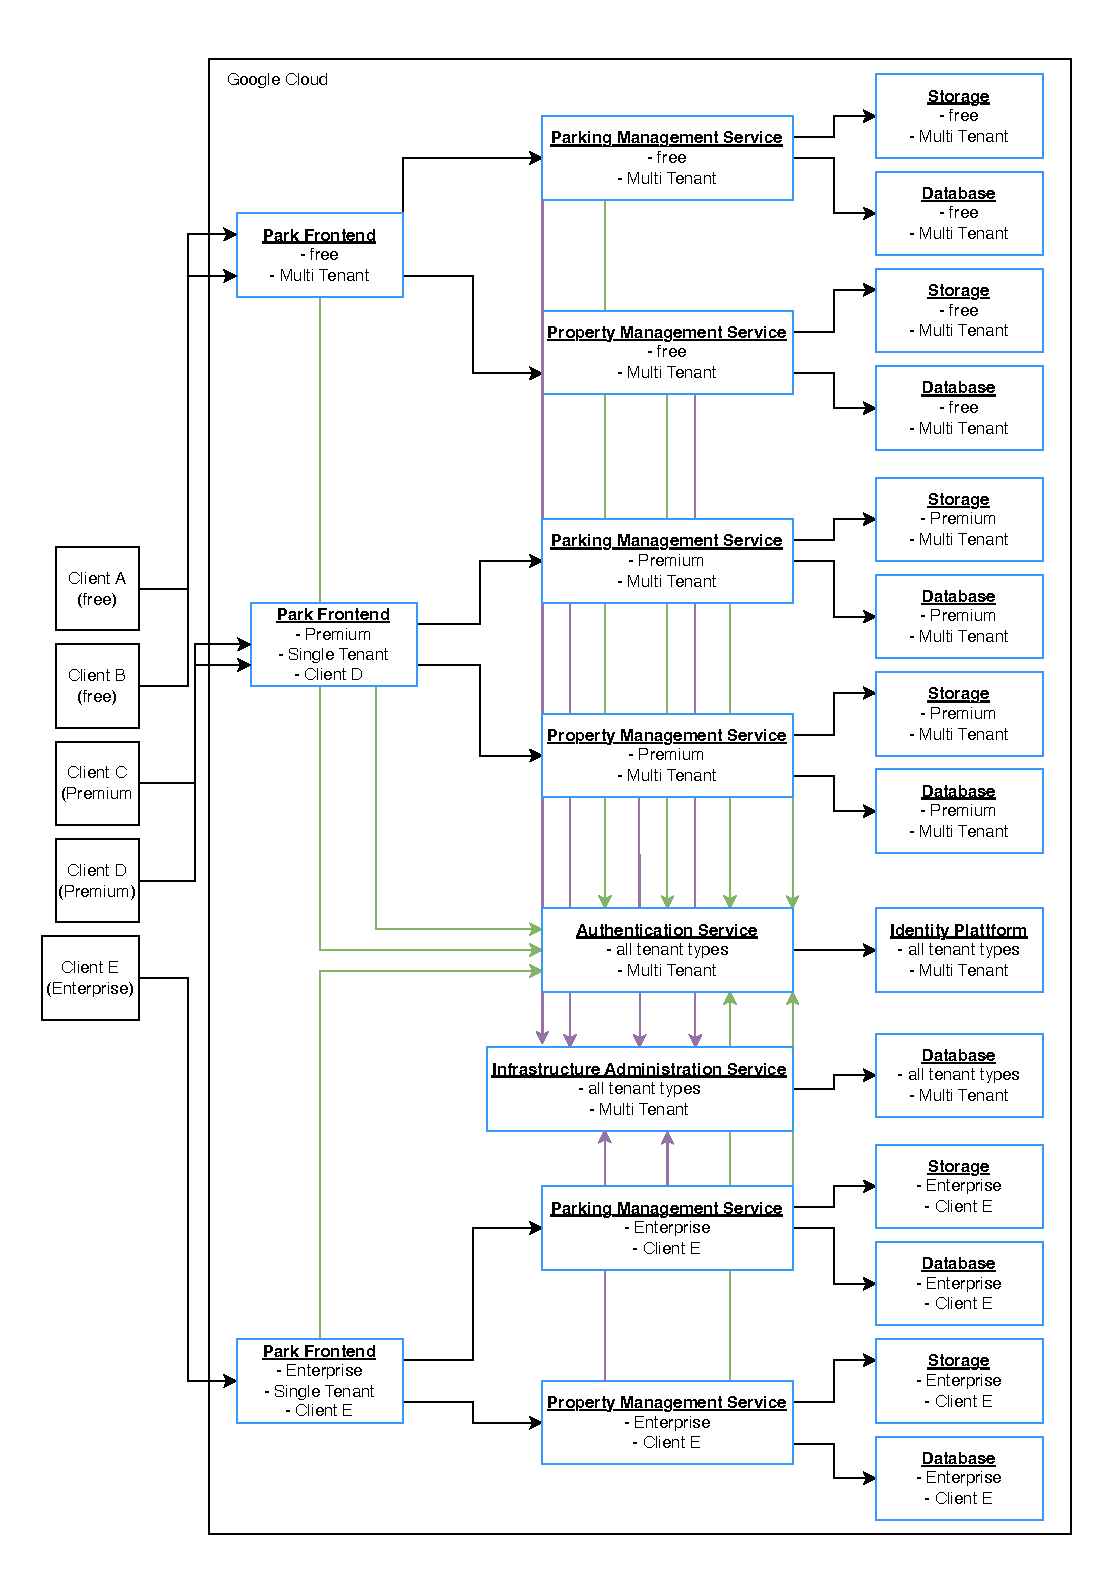
\includegraphics[width=0.95\textwidth]{resources/03-runtime-view/pdf/components-frontend-park.pdf}
	\caption{Alle verwendeten Komponenten, wenn ein Client mit dem Park Frontend interagiert, mit Berücksichtigung von Multitenancy}
	\label{fig:components-park-frontend}
\end{figure}

\begin{figure}[ht]
	\centering
	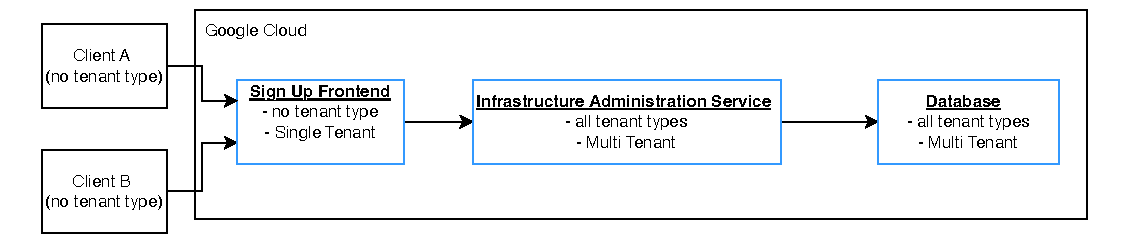
\includegraphics[width=\textwidth]{resources/03-runtime-view/pdf/components-frontend-signup.pdf}
	\caption{Alle verwendeten Komponenten, wenn ein Client mit dem Signup Frontend interagiert}
	\label{fig:components-signup-frontend}
\end{figure}

\subsection{Microservices}
Im Folgenden gehen wir nun auf die einzelnen Microservices ein, welche in Abbildung~\ref{fig:system-architecture} nochmal übersichtlich mit Components und Runtime Environment aufgelistet sind.
Auf die Components und das Runtime Environment wird hierbei nicht weiter eingegangen, da diese in den Abbildungen~\ref{fig:components-park-frontend}, \ref{fig:system-architecture} und~\ref{fig:components-signup-frontend} vollständig dargestellt sind.

\subsubsection{Globale Microservices}
Folgende Microservices werden von allen Tenants gemeinsam genutzt und werden in Google Cloud Run gehostet:

\paragraph{Sign Up Frontend}
\begin{itemize}
	\item Wird von allen Nutzern verwendet, um sich für einen neuen Tenant zu registrieren.
	\item Wird mittels Environment-Variablen konfiguriert. Die Environment-Variablen sind in Tabelle~\ref{tab:signup-frontend-env-vars} aufgelistet.
	\item Skaliert automatisch, da es in Google Cloud Run gehostet wird mit den Default Scaling Einstellungen.
	\item Der Microservice ist nicht customizable.
	\item Security Setup: Der Service hat und benötigt kein Security Setup, da er keinerlei Logik enthält und lediglich eine Request an den Infrastructure Management Service sender, wenn sich ein neuer Tenant registriert hat.
	\item Der Service kommuniziert lediglich mit einem Endpunkt des Infrastructure Management Services.
\end{itemize}

\paragraph{Authentication Service}
\begin{itemize}
	\item Wird verwendet um neue Nutzer und Tenants zu erstellen und um Informationen über Nutzer abzufragen.
	\item Wird mittels Environment-Variablen konfiguriert. Die Environment-Variablen sind in Tabelle~\ref{tab:auth-service-env-vars} aufgelistet.
	\item Skaliert automatisch, da es in Google Cloud Run gehostet wird mit den Default Scaling Einstellungen.
	\item Der Microservice ist nicht customizable.
	\item Security Setup: Der Microservice ist über HTTPS erreichbar und jeder einzelnen Anfrage muss ein Authorization Header angefügt werden (), in welchem das Identity Plattform JWT Token zur Validierung hinterlegt sein muss. Es ist mittels IAM Policy eingestellt, dass nur der Authentication Service auf die Authentication Firestore Datenbanken zugreifen kann.
	\item Der Microservice hat eine Verbindung zu seiner eigenen Authentication Firestore Datenbank und der Google Cloud Identity Platform.
\end{itemize}

\paragraph{Infrastructure Management Service}
\begin{itemize}
	\item Wird verwendet um neue Tenants zu erstellen, um Informationen über Tenants abzufragen und Analytics bezüglich Tenants zu speichern.
	\item Wird mittels Environment-Variablen konfiguriert. Die Environment-Variablen sind in Tabelle~\ref{tab:infra-admin-service-env-vars} aufgelistet.
	\item Skaliert automatisch, da es in Google Cloud Run gehostet wird mit den Default Scaling Einstellungen.
	\item Der Microservice ist nicht customizable.
	\item Security Setup: Der Microservice ist über HTTPS erreichbar und jeder einzelnen Anfrage muss ein Authorization Header angefügt werden, in welchem das Identity Plattform JWT Token zur Validierung hinterlegt sein muss. Es ist mittels IAM Policy eingestellt, dass nur der Infrastructure Management Service auf die Infrastructure Management Firestore Datenbanken und Infrastructure Management Cloud Storage Bucket zugreifen kann.
	\item Der Microservice hat eine Verbindung zu seiner eigenen Infrastructure Firestore Datenbank, seinem eigenen Cloud Storage Bucket und zu GitHub um die Pipelines zum Anlegen von neuen Tenants zu triggern.
\end{itemize}

\subsubsection{Tenant Typ spezifische Microservices}
Folgende Microservices werden von allen Tenants eines Tenant Typs gemeinsam genutzt. Pro Tenant Typ gibt es einen eigenen Namespace in der Google Cloud Kubernetes Engine, in welchem die Services laufen. Besonderheit ist hier der Enterprise Tenant Typ, welcher pro Tenant einen eigenen Namespace hat und deswegen die Services in diesem Abschnitt auch nicht geteilt werden.

\paragraph{Park Frontend}
\begin{itemize}
	\item Wird verwendet um neue Parkhäuser mit Parkplätzen und Ladestationen zu erstellen, um Informationen über Parkhäuser abzufragen, um Defects zu melden und Analytics zu betrachten.
	\item Wird mittels Environment-Variablen konfiguriert. Die Environment-Variablen sind in Tabelle~\ref{tab:park-frontend-env-vars} aufgelistet.
	\item Skaliert %TODO: @Benner Scaling
	\item Der Microservice ist nicht customizable. Das Frontend von Premium und Enterprise Tenants unterscheidet sich jedoch in der Darstellung, denn es gibt eine Analyticsseite und man kann zwischen den Sprachen Deutsch und Englisch wechseln.
	\item Security Setup: Die Nutzer müssen sich über die Identity Platform authentifizieren und der Service ist über HTTPS erreichbar. Es wird durch eine Anfrage an den Authentication Service sichergestellt, dass sich nur Nutzer des richtigen Tenant Typs in der jeweiligen Instanz anmelden können. Alle Anfragen an den Backend Service müssen ein Authorization Header mit dem Identity Platform JWT Token enthalten, damit nur authentifiziert Anfragen geschickt werden können. Alle Routen bis auch Home und Contact sind nur für authentifizierte Nutzer erreichbar.
	\item Der Service mit allen anderen Mircoservices.
\end{itemize}

\paragraph{Parking Management Service}
\begin{itemize}
	\item Wird verwendet für die Kommuniaktion mit Schranken, Bezahlterminals, Ladestationen und bietet eine Schnittstelle für externe Monitore um den Belegungsstatus abzufragen.
	\item Wird mittels Environment-Variablen konfiguriert. Die Environment-Variablen sind in Tabelle~\ref{tab:parking-mgmt-service-env-vars} aufgelistet.
	\item Skaliert %TODO: @Benner Scaling
	\item Der Microservice ist nicht customizable.
	\item Security Setup: Der Service ist über HTTPS erreichbar und den meisten Anfragen muss ein Authorization Header angefügt werden, in welchem das Identity Plattform JWT Token zur Validierung hinterlegt sein muss. Ausnahme ist hier der Endpunkt zum Belegungsstatus der immer frei abgefragt werden kann für ein Parkhaus. Es ist mittels IAM Policy eingestellt, dass nur der Parking Management Service auf die Parking Management Firestore Datenbank zugreifen kann.
	\item Der Service hat eine Verbindung zu seiner eigenen Parking Management Firestore Datenbank und zum Property Management Service.
\end{itemize}

\paragraph{Property Management Service}
\begin{itemize}
	\item Wird verwendet um Informationen über Parkhäuser abzufragen, um Defects zu verwalten und um Bilder von Defects zu speichern.
	\item Wird mittels Environment-Variablen konfiguriert. Die Environment-Variablen sind in Tabelle~\ref{tab:property-mgmt-service-env-vars} aufgelistet.
	\item Skaliert %TODO: @Benner Scaling
	\item Der Microservice ist nicht customizable.
	\item Security Setup: Der Service ist über HTTPS erreichbar und für alle Anfragen muss ein Authorization Header angefügt werden, in welchem das Identity Plattform JWT Token zur Validierung hinterlegt sein muss. Es ist mittels IAM Policy eingestellt, dass nur der Property Management Service auf die Property Management Firestore Datenbank und den Property Management Cloud Storage Bucket zugreifen kann.
	\item Der Service hat eine Verbindung zu seiner eigenen Property Management Firestore Datenbank, seinem eigenen Cloud Storage Bucket und zum Parking Management Service.
\end{itemize}

\subsection{Data Stores}

\subsubsection{Globale Datastores}
Folgende Datastores werden von den globalen Cloud Run Microservices genutzt:

\paragraph{Authentication Firestore}
\begin{itemize}
	\item Wird verwendet um durch den Authentication Service Nutzer zu speichern.
	\item Integrity Constraints: Die Nutzer Id, welche durch Identity Platform generiert wird, ist eindeutig und wird als Primärschlüssel verwendet.
	\item Security Constraints: Nur der Authentication Service hat Zugriff (IAM Policy) auf die Datenbank.
\end{itemize}

\paragraph{Infrastructure Management Firestore}
\begin{itemize}
	\item Wird verwendet um für die Abrechnung die Anzahl der Requests des Tenants abzuspeichern und Daten für Analytics pro Tenant zu sammeln..
	\item Integrity Constraints: Die Tenant Id, welche durch Identity Platform generiert wird, ist eindeutig und wird als Primärschlüssel verwendet.
	\item Security Constraints: Nur der Infrastructure Management Service hat Zugriff (IAM Policy) auf die Datenbank.
\end{itemize}

\paragraph{Infrastructure Management Cloud Storage Bucket}
\begin{itemize}
	\item Wird verwendet um für die Abrechnung die Anzahl der Requests des Tenants abzuspeichern und Daten für Analytics pro Tenant zu sammeln.
	\item Integrity Constraints: Die Tenant Id, welche durch Identity Platform generiert wird, ist eindeutig und wird als Primärschlüssel verwendet.
	\item Security Constraints: Nur der Infrastructure Management Service hat Zugriff (IAM Policy) auf den Bucket.
\end{itemize}

\subsubsection{Tenant Typ spezifische Datastores}
Folgende Datastores werden von einem Tenant Typ spezifischen Kubernetes Namespace genutzt. Auch hier ist es wieder so, dass der Enterprise Tenant Typ pro Tenant einen eigenen Namespace hat und deswegen die Datastores in diesem Abschnitt auch nicht geteilt werden.

\paragraph{Parking Management Firestore}
\begin{itemize}
	\item Wird verwendet um Informationen Ladevorgänge, Parkhausbelege usw. zu speichern.
	\item Integrity Constraints: Die Parkhaus Id, welche durch den Property Management Service generiert wird, ist eindeutig und wird als Primärschlüssel verwendet. Für alle untergeordneten Collections und Daten werden auch eindeutige Primärschlüssel verwendet.
	\item Security Constraints: Nur der Parking Management Service hat Zugriff (IAM Policy) auf die Datenbank.
\end{itemize}

\paragraph{Property Management Firestore}
\begin{itemize}
	\item Wird verwendet um Informationen über Parkhäuser und Defects abzuspeichern.
	\item Integrity Constraints: Die Parkhaus Id und Defect Id, welche durch den Property Management Service generiert wird, ist eindeutig und wird als Primärschlüssel verwendet.
	\item Security Constraints: Nur der Property Management Service hat Zugriff (IAM Policy) auf die Datenbank.
\end{itemize}

\paragraph{}